{ %section2_2
	\subsection{Метод Амдала}
	\parПри оценке эффективности распараллеливания некоторой программы, выполняющей фиксированный объём работы, скорость выполнения можно выразить следующим образом:$\left.V(p)\right|_{w=const}\;=\;\frac w{t(p)}$, где $w$ – это общее количество УЕР, содержащихся в рассматриваемой программе, $t(p)$ – время выполнения работы w при использовании $p$ процессоров. Тогда выражение для параллельного ускорения примет вид:
	\begin{equation}
		\label{AmdalSFromP:equation}
		\left.S(p)\right|_{w=const}\;=\;\frac{V(p)}{V(1)}\;=\;\frac w{t(p)}\;=\;\frac w{t(1)}\;=\;\frac{t(1)}{t(p)}.
	\end{equation}
	\parЗапишем время $t(1)$ следующим образом:
	\begin{equation}
		t(1)\;=\;t(1)\;+\;(k\;\cdot\;t(1)\;-\;k\;\cdot\;t(1))\;=\;k\;\cdot\;t(1)\;+\;(1\;-\;k)\;\cdot\;t(1),
	\end{equation}
	где $k\;\in\;\lbrack0,1)$ - это коэффициент распараллеленности программы, которым мы обозначим долю времени, в течение которого выполняется идеально распараллеленный код внутри рассматриваемой программы. Такой код можно выполнить ровно в $p$ раз быстрее, если количество процессоров увеличить в p раз. Заметим, что коэффициент $k$ никогда не равен единице, т.к. в любой программе всегда присутствует нераспараллеливаемый код, который приходится выполнять последовательно на одном процессоре (ядре), даже если их доступно несколько. Если для некоторой программы $k=0$, то при запуске этой программы на любом количестве процессоров $p$ она будет решаться за одинаковое время.
	\parУчитывая, что в методе Амдала количество работы остаётся неизменным при любом $p$ (т.к. $w=const$), можно утверждать, что значение $k$ не изменяется в проводимых экспериментах, следовательно можем записать:
	\begin{equation}
		\label{AmdalTFromP:equation}
		t(p)\;=\;\frac{k\;\cdot\;t(1)}p\;+\;(1\;-\;k)\;\cdot\;t(1),
	\end{equation}
	где первое слагаемое даёт время работы распараллеленного в p раз идеально распараллеливаемого кода, а второе слагаемое – время работы нераспараллеленного кода, которое не меняется при любом $p$. Подставив формулу~\eqref{AmdalTFromP:equation} в~\eqref{AmdalSFromP:equation}, получим выражение $$\left.S(p)\right|_{w=const}\;=\;\frac{t(1)}{t(p)}\;=\;\frac{t(1)}{{\displaystyle\frac{k\;\cdot\;t(1)}p}\;+\;(1\;-\;k)\;\cdot\;t(1)}\;=\;\frac1{{\displaystyle\frac kp}\;+\;1\;-\;k},$$ которое перепишем в виде
	\begin{equation}
		\label{AmdalLaw:equation}
		\left.S(p)\right|_{w=const}\;=\;S_A(p)\;=\;\left(\frac kp\;+\;1\;-\;k\right)^{-1}
	\end{equation}
	более известном как \textbf{закон Амдала} – по имени американского учёного Джина Амдала, предложившего это выражение в 1967 году. До сих пор в специализированной литературе по параллельным вычислениям именно этот закон является основополагающим, т.к. позволяет получить теоретическое ограничение сверху для скорости выполнения некоторой заданной программы при распараллеливании.
	\parГрафик зависимости параллельного ускорения от количества ядер изображен на рисунке~\ref{GraphAmdalSFromP:image}:
	\begin{figure}[H]
		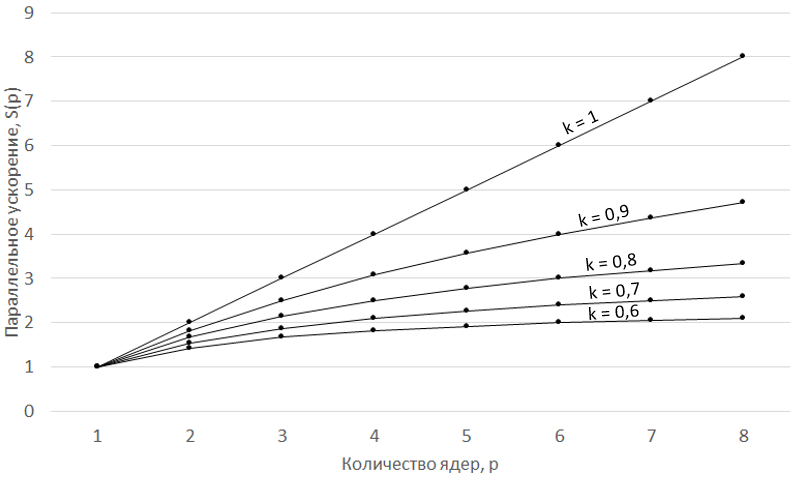
\includegraphics[width=1\linewidth]{GraphAmdalSFromP}
		\caption{\textit{График зависимости параллельного ускорения от количества ядер по Амдалу}}
		\label{GraphAmdalSFromP:image}
	\end{figure}
	\parОтметим, что выражение для расчёта параллельной эффективности при использовании метода Амдала можно получить, объединив формулы~\eqref{parallelEffect:equation} и~\eqref{AmdalLaw:equation}, а именно:
	\begin{equation}
		E_A(p)\;=\;\left(k\;+\;p\;-\;p\;\cdot\;k\right)^{-1}
	\end{equation}
	\parВажным допущением закона Амдала является идеализация физического смысла величины $k$, состоящая в предположении, что идеально распараллеленный код будет давать линейный прирост скорости работы при изменении $p$ от $0$ до $+\infty$ . При решении реальных задач приходится ограничивать этот интервал сверху некоторым конечным положительным значением $p_{max}$ и/или исключать из этого интервала все значения, не кратные некоторой величине, обычно задающей размерность задачи.
	\parНапример, код программы, выполняющей конволюционное кодирование независимо для пяти равноразмерных файлов, может давать линейное ускорение при изменении $p$ от $1$ до $5$, но уже при $p=6$ скорее всего покажет нулевой прирост скорости выполнения задачи (по сравнению с решением при $p=5$). Это объясняется тем, что  конволюционное кодирование, также известно как ''свёрточное'', является принципиально нераспараллеливаемым при кодировании выбранного блока данных.
	\par
}